% PROPOSTA B (05/11/2026, pedido do autor) para substituir o Quadro 3: um
% gráfico de barras com o número de configurações de cada forma de uso do GARCH
% e a conta que o gera. Fora do TG até o autor decidir. Contagens do Quadro 3,
% conferidas nos dados/resultados/refeito_2026-10-05/grades/r3_*.txt.
\documentclass[10pt,border=2pt]{standalone}
\usepackage[T1]{fontenc}
\usepackage[utf8]{inputenc}
\usepackage{mathptmx}
\usepackage{pgfplots}
\pgfplotsset{compat=1.18}
\begin{document}
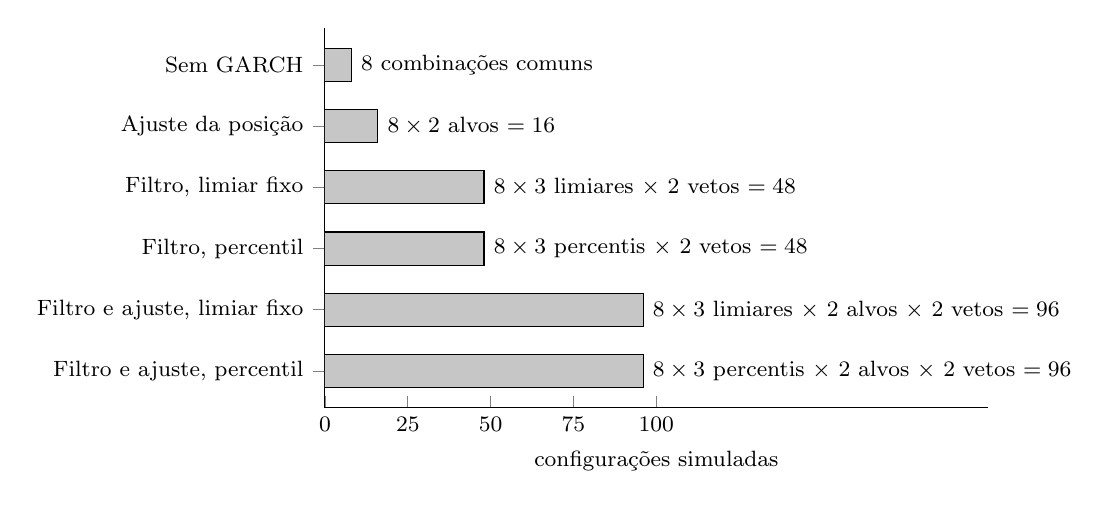
\begin{tikzpicture}
\begin{axis}[
  xbar, width=10cm, height=6.4cm, bar width=4.2mm,
  xmin=0, xmax=200, axis x line*=bottom, axis y line*=left,
  xlabel={configurações simuladas}, xlabel style={font=\footnotesize},
  ytick=data, y dir=reverse,
  yticklabels={Sem GARCH, Ajuste da posição, {Filtro, limiar fixo}, {Filtro, percentil},
               {Filtro e ajuste, limiar fixo}, {Filtro e ajuste, percentil}},
  yticklabel style={font=\footnotesize, align=right},
  xtick={0,25,50,75,100}, tick label style={font=\footnotesize},
  enlarge y limits=0.12,
  nodes near coords, point meta=explicit symbolic,
  every node near coord/.append style={font=\footnotesize, anchor=west},
]
\addplot[draw=black, fill=gray!45] coordinates {
  (8,1)  [8 combinações comuns]
  (16,2) [$8 \times 2$ alvos $= 16$]
  (48,3) [$8 \times 3$ limiares $\times\ 2$ vetos $= 48$]
  (48,4) [$8 \times 3$ percentis $\times\ 2$ vetos $= 48$]
  (96,5) [$8 \times 3$ limiares $\times\ 2$ alvos $\times\ 2$ vetos $= 96$]
  (96,6) [$8 \times 3$ percentis $\times\ 2$ alvos $\times\ 2$ vetos $= 96$]
};
\end{axis}
\end{tikzpicture}
\end{document}
